\documentclass[intlimits, 9pt, unicode]{beamer} 

\usepackage[T2A]{fontenc}
%\usepackage[cp1251]{inputenc}
\usepackage[utf8]{inputenc}
\usepackage[russian]{babel}
\usepackage{graphicx}
\usepackage{amssymb}
\usepackage{amsthm}

\usefonttheme[onlymath]{serif}

\usepackage{beamerthemesplit}

\usetheme{Warsaw}

\setbeamerfont{institute}{size=\normalsize}

\setbeamercolor{bluetext_color}{fg=blue}
\newcommand{\bluetext}[1]{{\usebeamercolor[fg]{bluetext_color}#1}}

\setbeamercovered{transparent}

\title{Change point detection in mobile advertising}
\author{Nina Golyandina, Kliment Merzlyakov}
\institute{Saint Petersburg State University \\
    Mathematical faculty \\
     Applied statistics department \\
}
\date{
    Saint Petersburg\\
    2018
}

\AtBeginSection[]{
  \begin{frame}
  \vfill
  \centering
  \begin{beamercolorbox}[sep=8pt,center,shadow=true,rounded=true]{title}
    \usebeamerfont{title}\insertsectionhead\par%
  \end{beamercolorbox}
  \vfill
  \end{frame}
}

\begin{document}

\begin{frame}
    \titlepage
\end{frame}

\begin{frame}
    \frametitle{Content}

    \begin{itemize}
    	\item Change point detection
		     	 \begin{itemize}
	    		   \item What is change point detection?
		    	   \item Real world examples of change point detection 
		    	   \item Reasons to detect change points
		    	  \end{itemize}
        \item Change point detection techniques
        \item Airpush cases
		     	 \begin{itemize}
	    		   \item Fraud elimination
		    	   \item Trend extraction
		    	   \item Smart alerts
		    	  \end{itemize}
    \end{itemize}
\end{frame}

\section{Change point detection}

\begin{frame}
    \frametitle{What is change point detection?}

    \begin{itemize}
    	\item Change point --- point in time series where some significant change occurred
	\item Change point detection --- group of methods to find change points in time series
	\item Change points can be two types:
		\begin{itemize}
			\item Local --- one time change
			\item Global --- change of time series structure 
		\end{itemize}
    \end{itemize}
\end{frame}

\begin{frame}
    \frametitle{What is change point detection?}

Let's formalize change point detection problem:
    \begin{itemize}
	\item Suppose $\mathrm{X} = (x_1, ..., x_N)$ --- time series of length $N$
	\item $\mathbf{t} = \{t_1,t_2,...\} \subset \{1,...,K\}$ --- set of change points indexes
	\item $K-1$ --- amount of changes in time series, which can be either known or unknown
	\item Change point detection problem --- is a problem of searching such set of indexes, which would be the closest to real set of change point indexes: $\widehat{\mathbf{t}} = \{\widehat{t_1},\widehat{t_2},...\} $
	\item To estimate change point detection algorithm quality we need tagged time series with known indexes $\widehat{\mathbf{t}} = \{\widehat{t_1},\widehat{t_2},...\} $
	\item Quality can be estimated as sum of distance between real indexes and estimated indexes normalized by length of time series: $$\sum_{i=1}^K \frac{|\widehat{t_i} - t_i|}{N}$$	
	
    \end{itemize}
\end{frame}

\begin{frame}
    \frametitle{Types of change points}

    \begin{itemize}
    	\item Trend change
	\item Mean change
	\item Variance change
	\item Single point change
	\item Period change
	\item Structure change
    \end{itemize}
\end{frame}

\begin{frame}
\frametitle{Change point examples}
\begin{figure}
\textbf{Common graph}\par\medskip
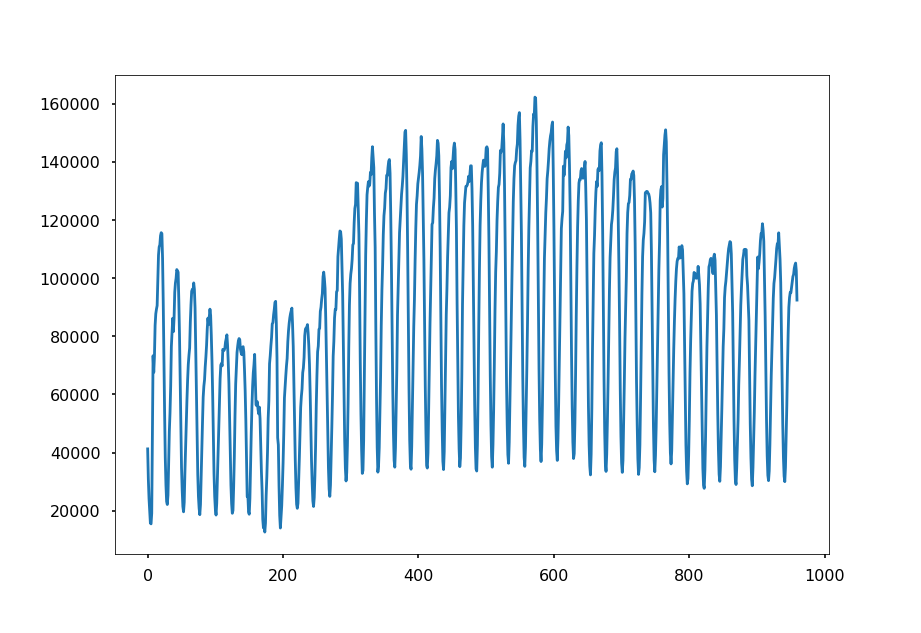
\includegraphics[scale=0.30]{images/001_normal_1}
\end{figure}
\end{frame}

\begin{frame}
\frametitle{Change point examples}
\begin{figure}
\textbf{Common graph with trend}\par\medskip
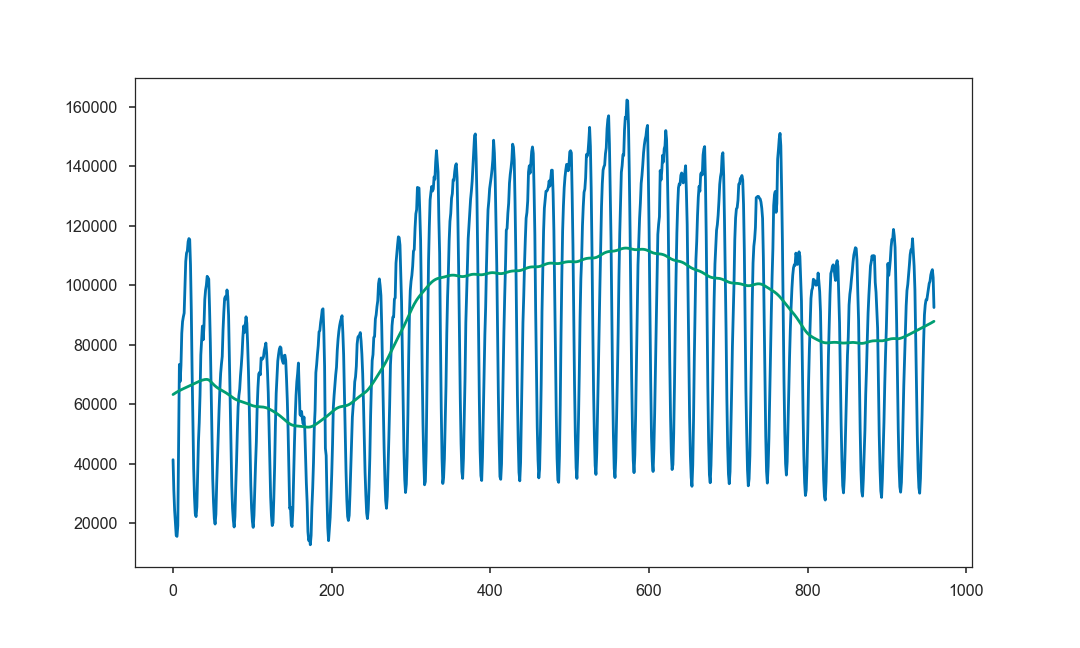
\includegraphics[scale=0.30]{images/001_normal_2}
\end{figure}
\end{frame}

\begin{frame}
\frametitle{Change point examples}
\begin{figure}
\textbf{Common graph without trend}\par\medskip
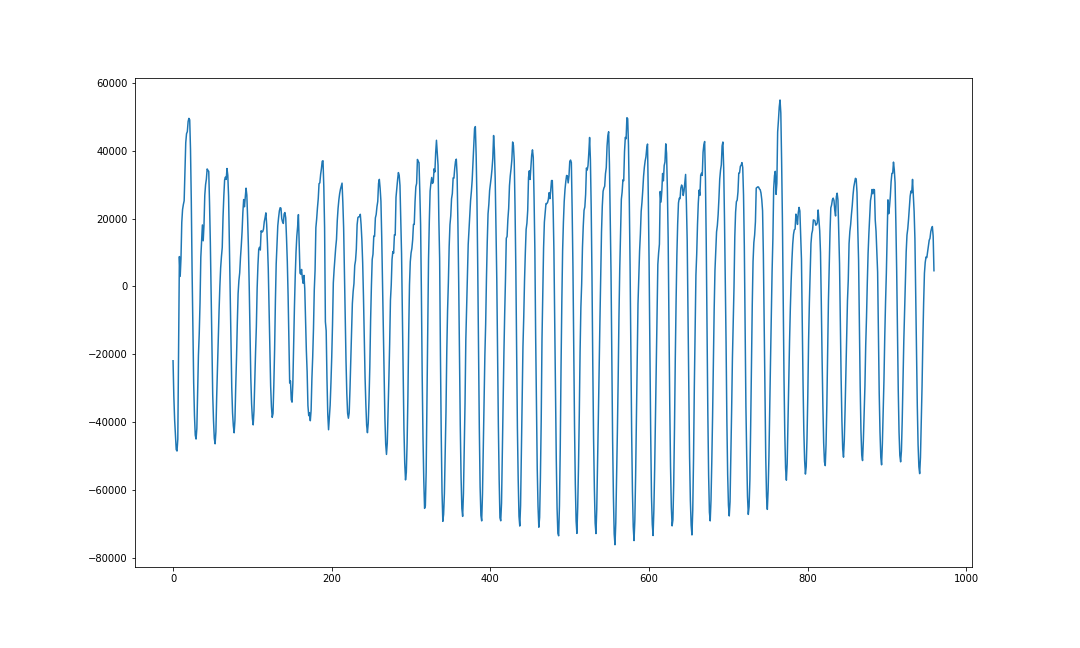
\includegraphics[scale=0.30]{images/001_normal_3}
\end{figure}
\end{frame}

\begin{frame}
\frametitle{Change point examples}
\begin{figure}
\textbf{Common graph periodic frequency}\par\medskip
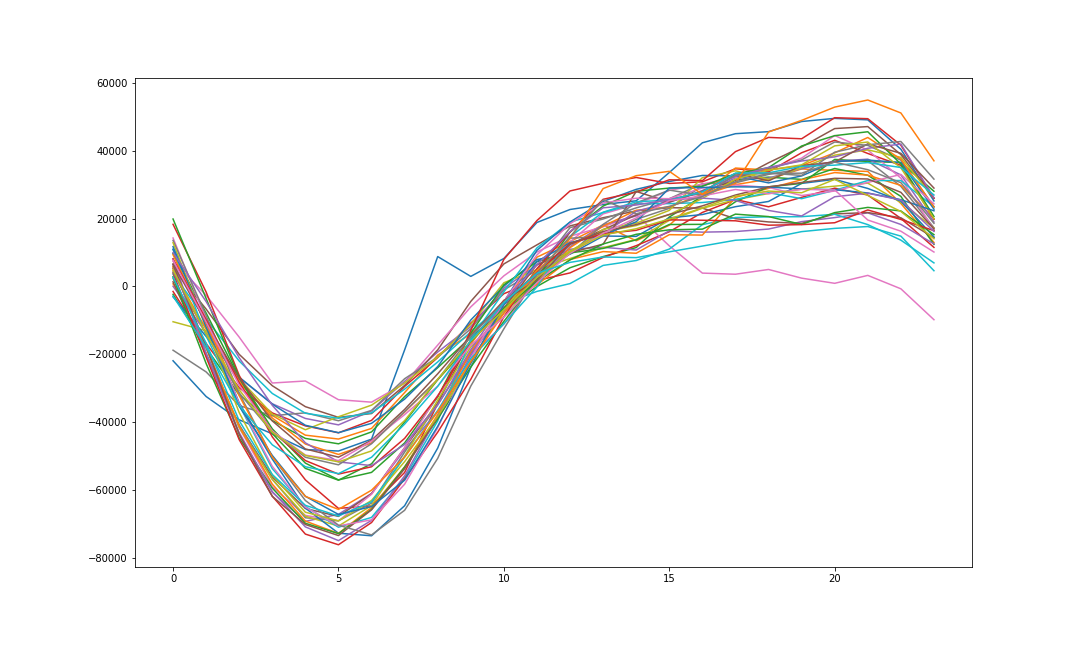
\includegraphics[scale=0.30]{images/001_normal_4}
\end{figure}
\end{frame}

\begin{frame}
\frametitle{Change point examples}
\begin{figure}
\textbf{Mean change}\par\medskip
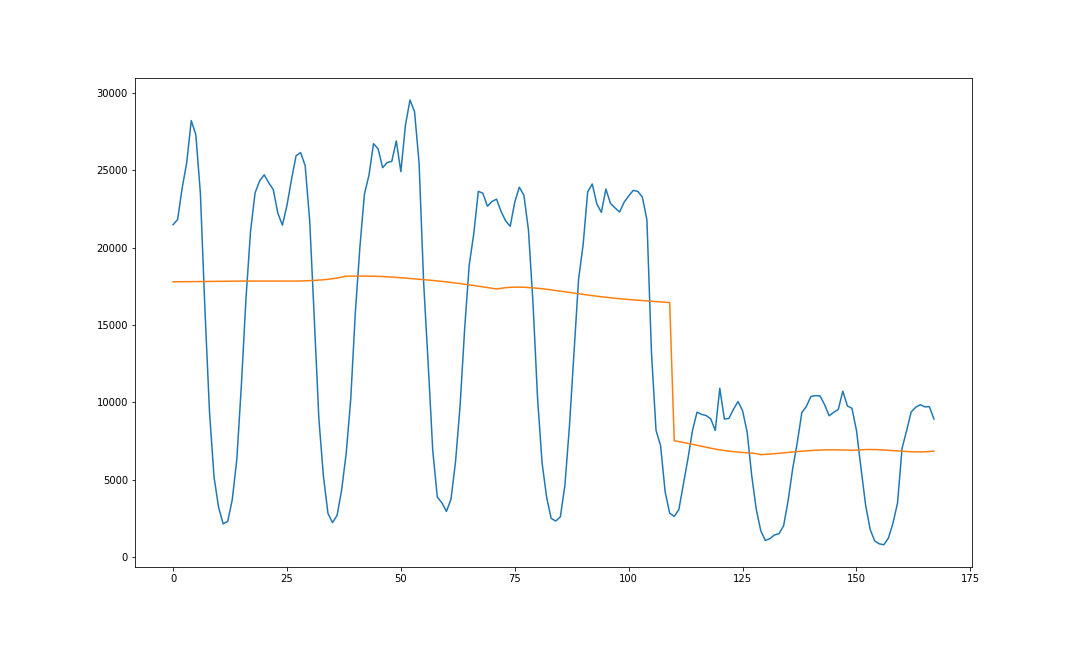
\includegraphics[scale=0.30]{images/002_mean}
\end{figure}
\end{frame}

\begin{frame}
\frametitle{Change point examples}
\begin{figure}
\textbf{Variance change}\par\medskip
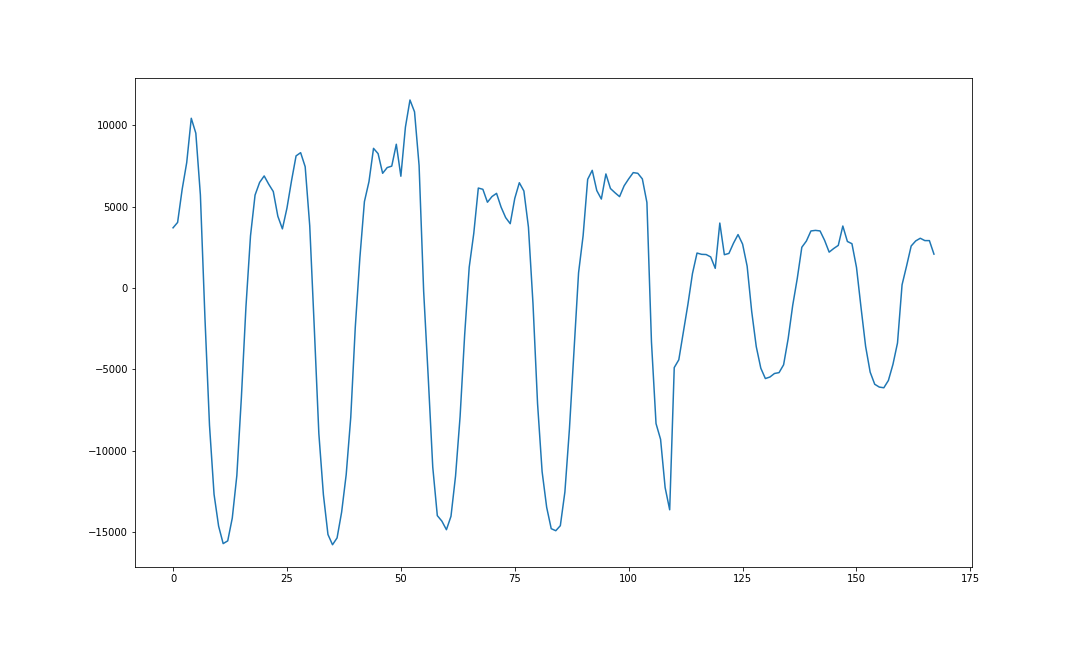
\includegraphics[scale=0.30]{images/003_variance}
\end{figure}
\end{frame}

\begin{frame}
\frametitle{Change point examples}
\begin{figure}
\textbf{Trend change}\par\medskip
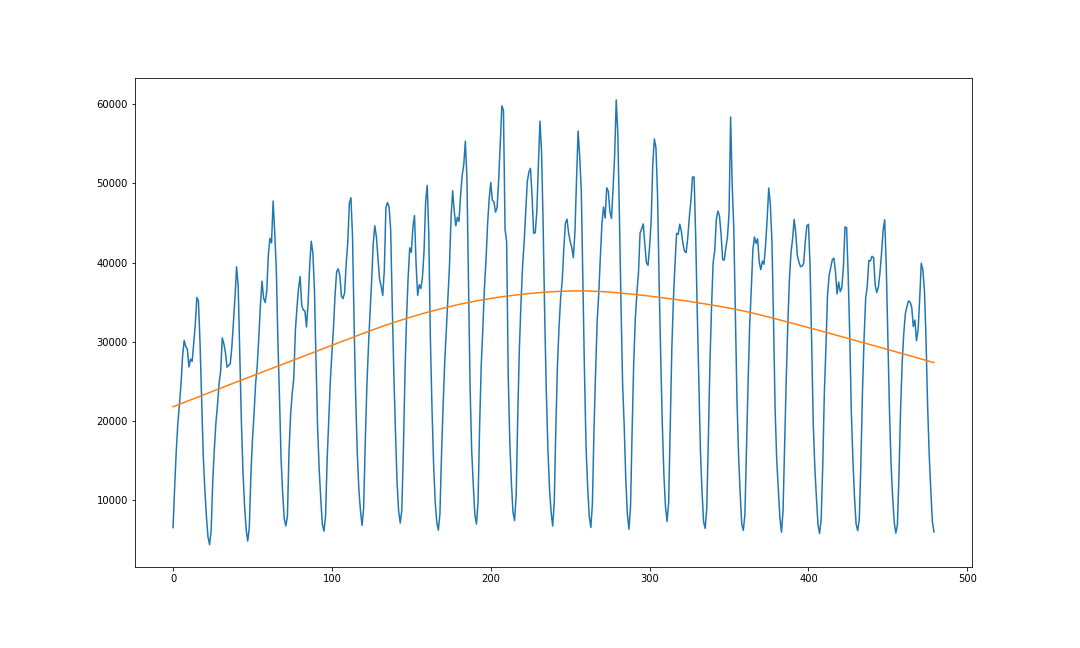
\includegraphics[scale=0.30]{images/004_trend}
\end{figure}
\end{frame}

\begin{frame}
\frametitle{Change point examples}
\begin{figure}
\textbf{Point change}\par\medskip
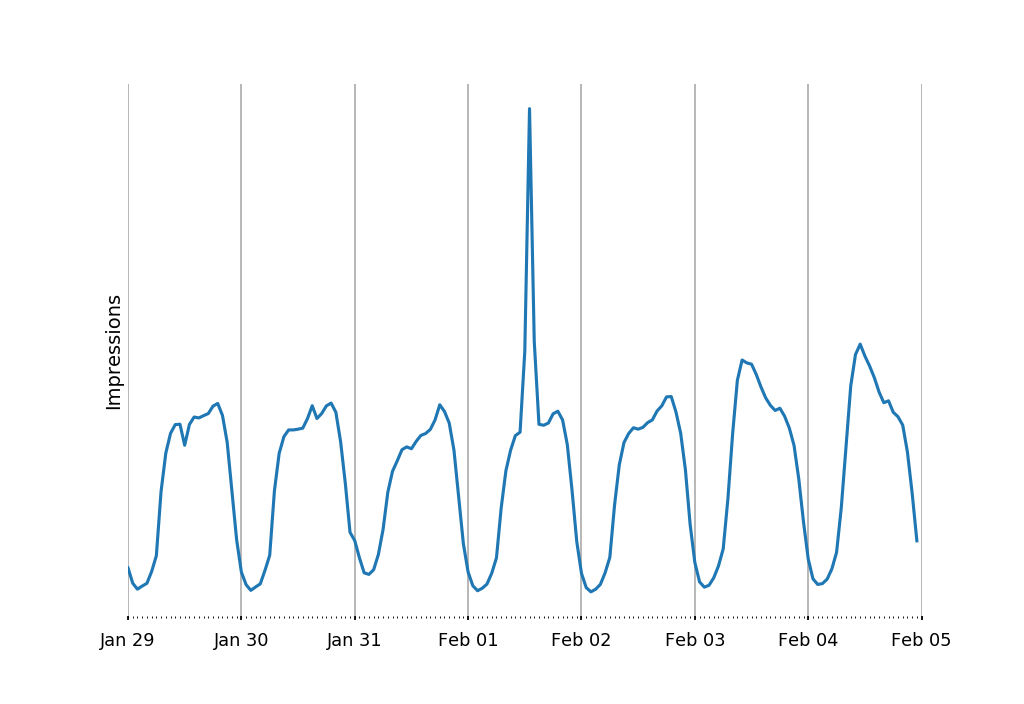
\includegraphics[scale=0.30]{images/005_point}
\end{figure}
\end{frame}

\begin{frame}
\frametitle{Change point examples}
\begin{figure}
\textbf{Structure change}\par\medskip
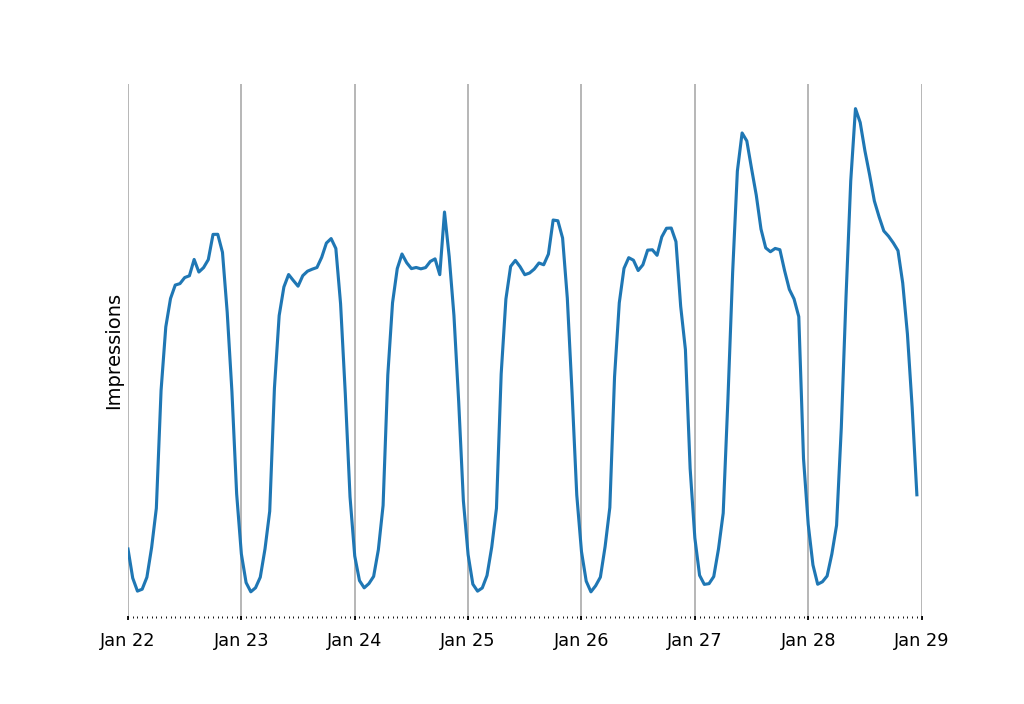
\includegraphics[scale=0.30]{images/006_structure}
\end{figure}
\end{frame}

\begin{frame}
    \frametitle{Reasons to detect change points}

    \begin{itemize}
    	\item Searching issues in historical data 
	\item Reacting on changes quickly
	\item Extracting trend more accurately
    \end{itemize}
\end{frame}


\section{Change point detection techniques}

\begin{frame}
    \frametitle{SSA for change point detection}

Singular spectrum analysis (SSA) method can be used to allocate change points.
Let $x_1,x_2,...$ be a time series and $N, L, l, p, q$ be fixed integers so that $0 \leq l < L \leq N/2$ and $ 0 \leq p < q$. The SSA change point detection algorithm is as follows.
For each $ n = 0,1,...$ we compute:
    \begin{itemize}
    	\item the base matrix $\mathbb{X}^{(n)}$,
	\item the lag-covariance matrix $\mathbb{R}_n = \mathbb{X}^{(n)}(\mathbb{X}^{(n)})^{\top}$,
	\item the SVD of $\mathbb{R}_n$,
	\item $\mathbf{\nu}_{n.I,p,q}$, the sum of the squared Euclidean distances between the vectors $\mathbb{X}_j^{(n)} (j = p+1,...,q$ and the l-dimensional subspace $L_{n,I}$, and
	\item $S_n$, the normalized squared distance.
    \end{itemize}
 Large values of $S_n$ indicate a change in the time series.

This method has the following parameters:
	\begin{itemize}
		\item $N$ --- window size for base matrix
		\item $L, I$ --- SSA window and number of eigenvectors
		\item $p, q$ --- window size for test matrix
		\item threshold
	\end{itemize}
\end{frame}

\begin{frame}
    \frametitle{SSA in action. Mean change}

Let's try to apply SSA algorithm to real time series mentioned above. With manually settled parameters.
\begin{figure}
	\textbf{Mean change}
	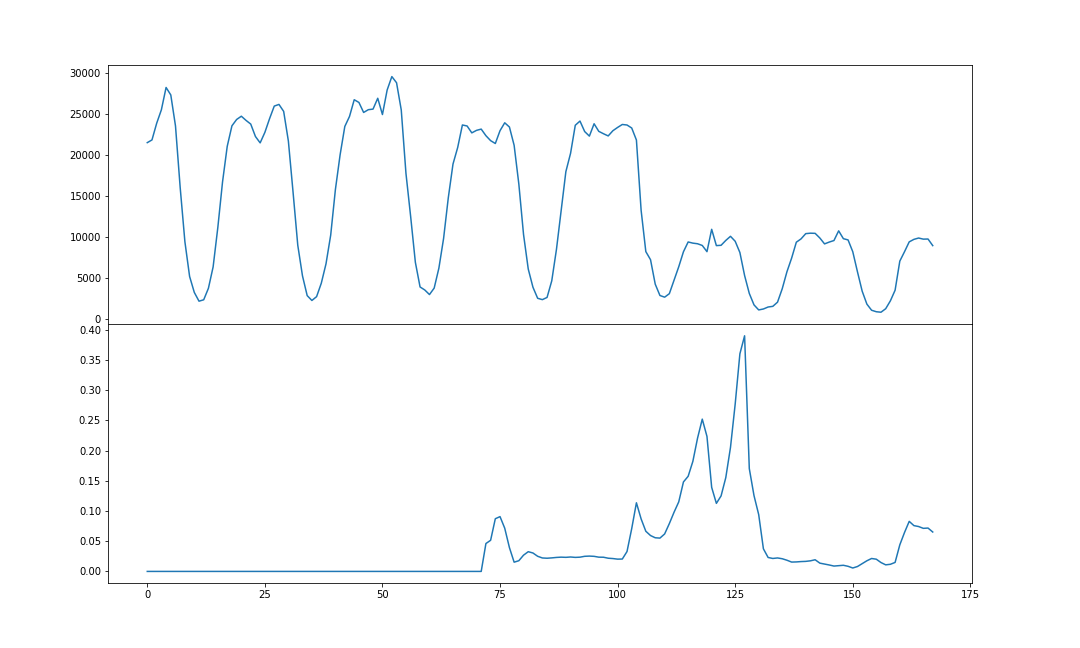
\includegraphics[scale=0.10]{images/017_mean_cp}
	\textbf{Detection}
	N = 48, L = 24, I = 5, p = 49, q = L, threshold = 0.15
	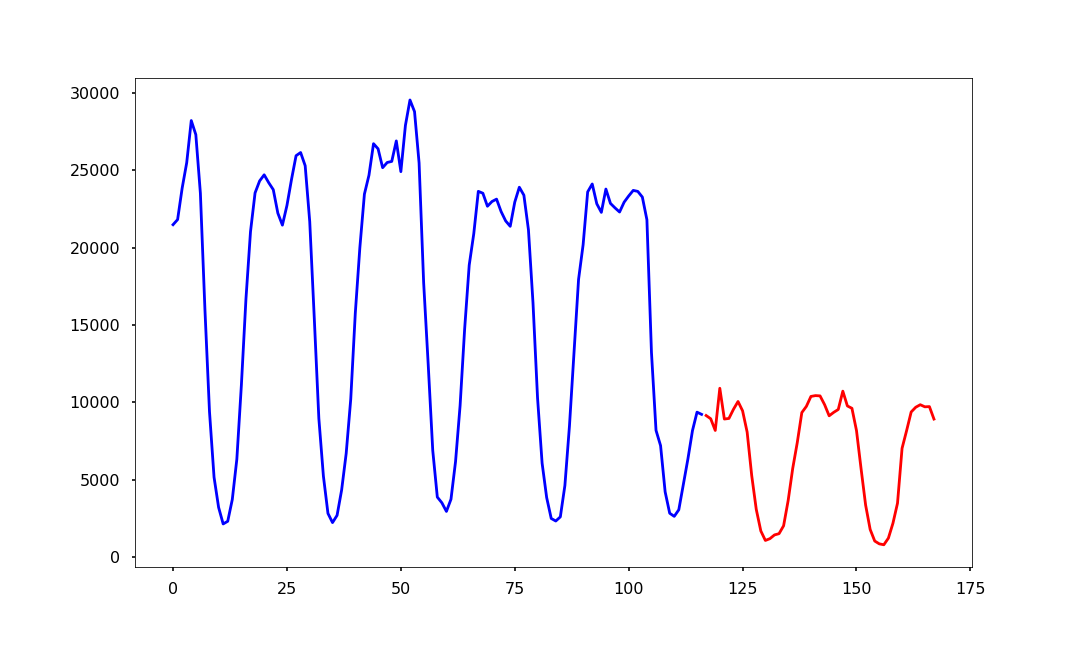
\includegraphics[scale=0.10]{images/018_mean_cp_detected}
\end{figure}

Works good for mean change

\end{frame}

\begin{frame}
    \frametitle{SSA in action. Variance change}

\begin{figure}
	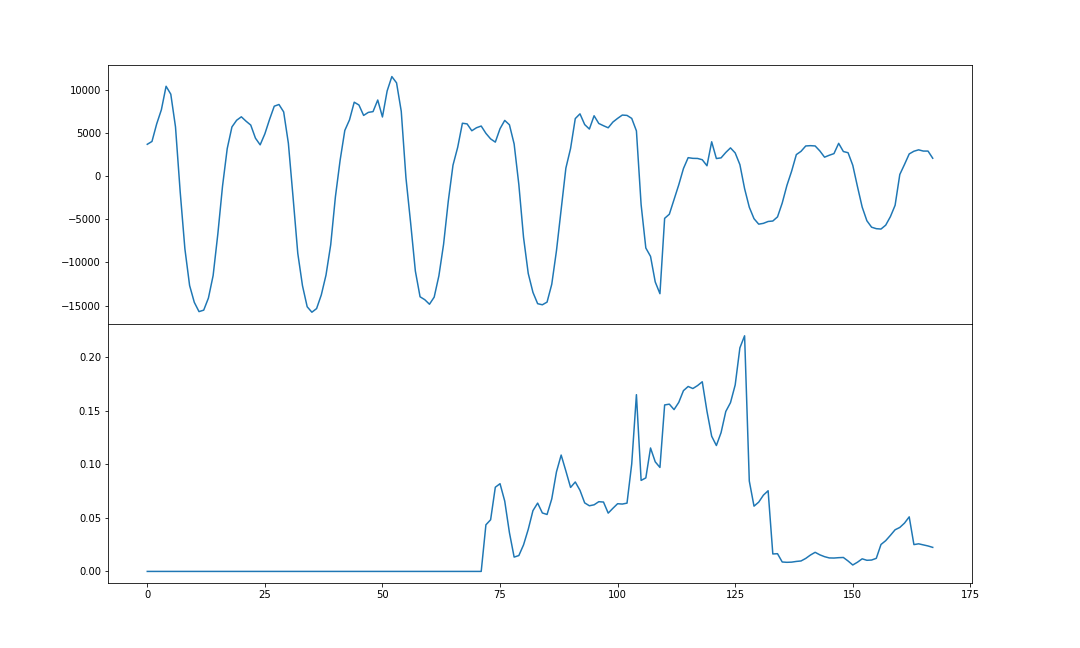
\includegraphics[scale=0.10]{images/019_variance_cp}
	N = 48, L = 24, I = 5, p = 49, q = L, threshold = 0.15
	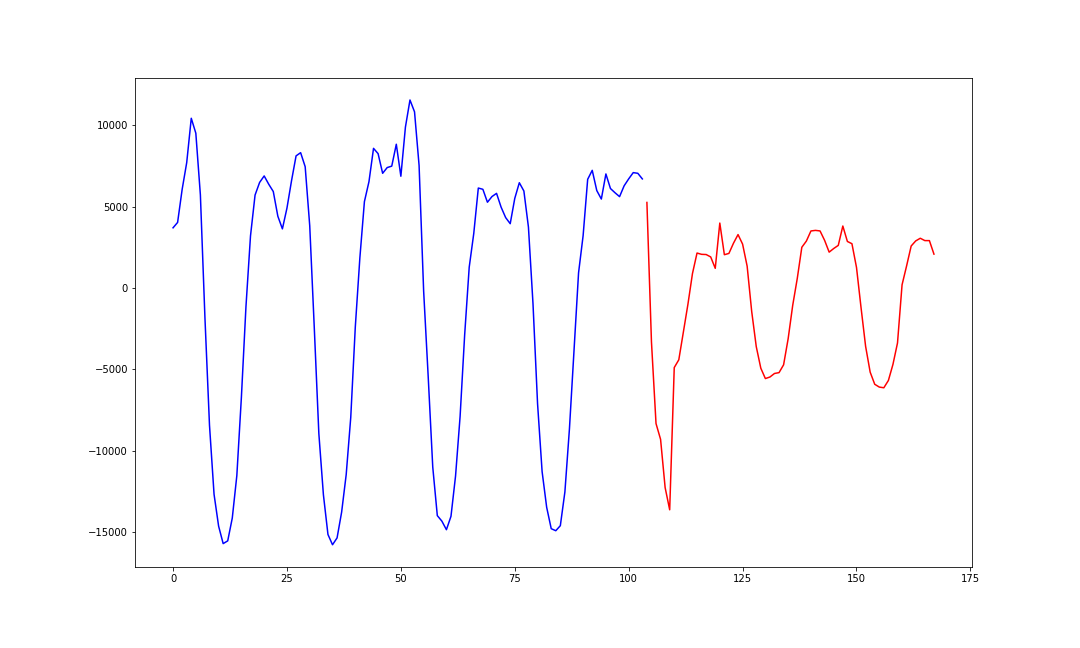
\includegraphics[scale=0.10]{images/020_variance_cp_detected}
\end{figure}

Works good for variance change

\end{frame}

\begin{frame}
    \frametitle{SSA in action. Period change}

\begin{figure}
	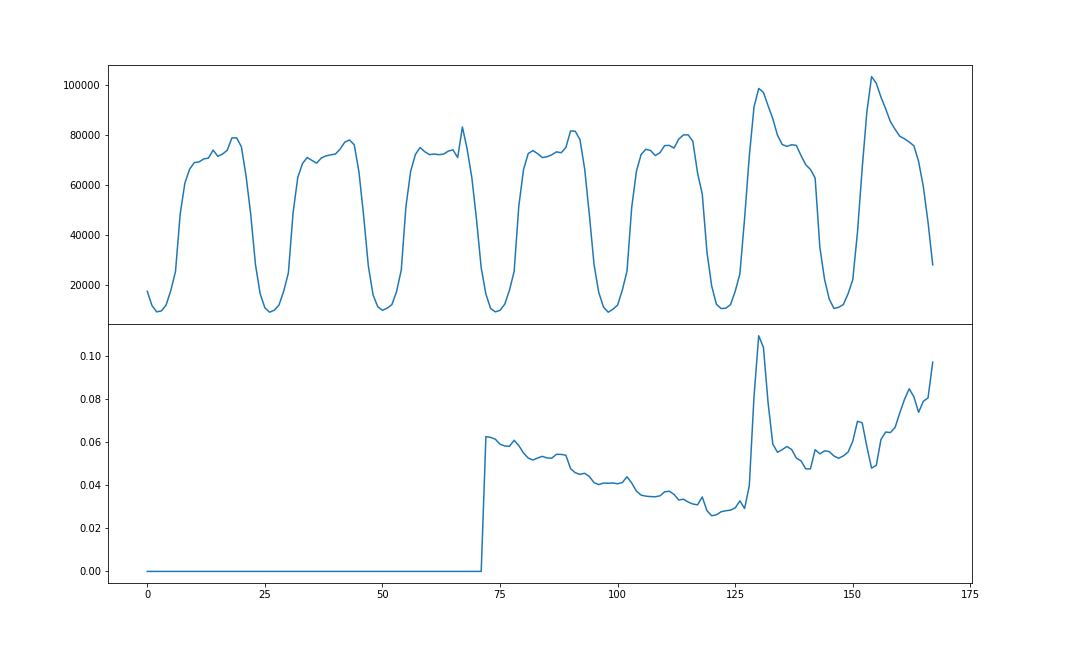
\includegraphics[scale=0.10]{images/025_period_cp}
	N = 48, L = 24, I = 5, p = 49, q = L, threshold = 0.1
	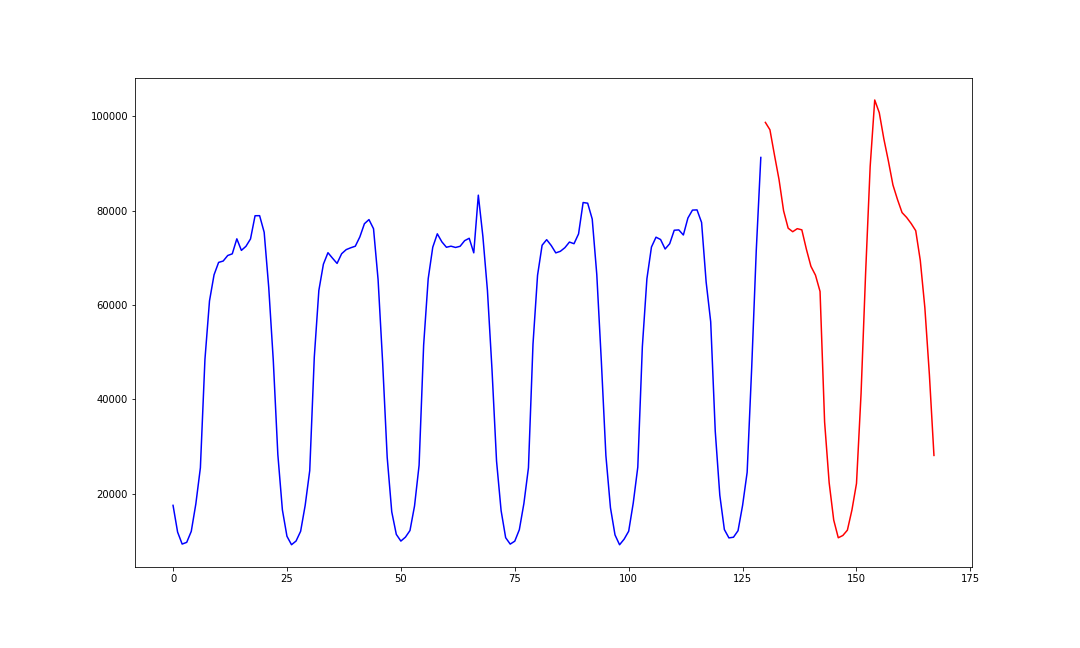
\includegraphics[scale=0.10]{images/026_period_cp_detected}
\end{figure}

Works well for period change

\end{frame}


\begin{frame}
    \frametitle{SSA in action. Point change}

\begin{figure}
	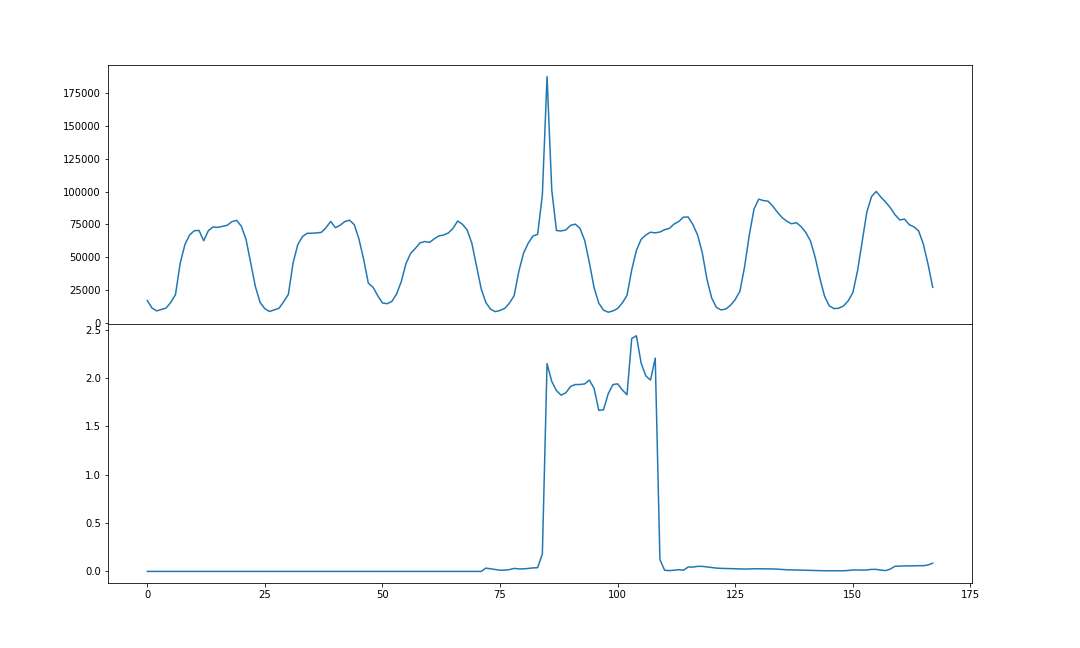
\includegraphics[scale=0.10]{images/021_point_cp}
	N = 48, L = 24, I = 5, p = 49, q = L, threshold = 0.1
	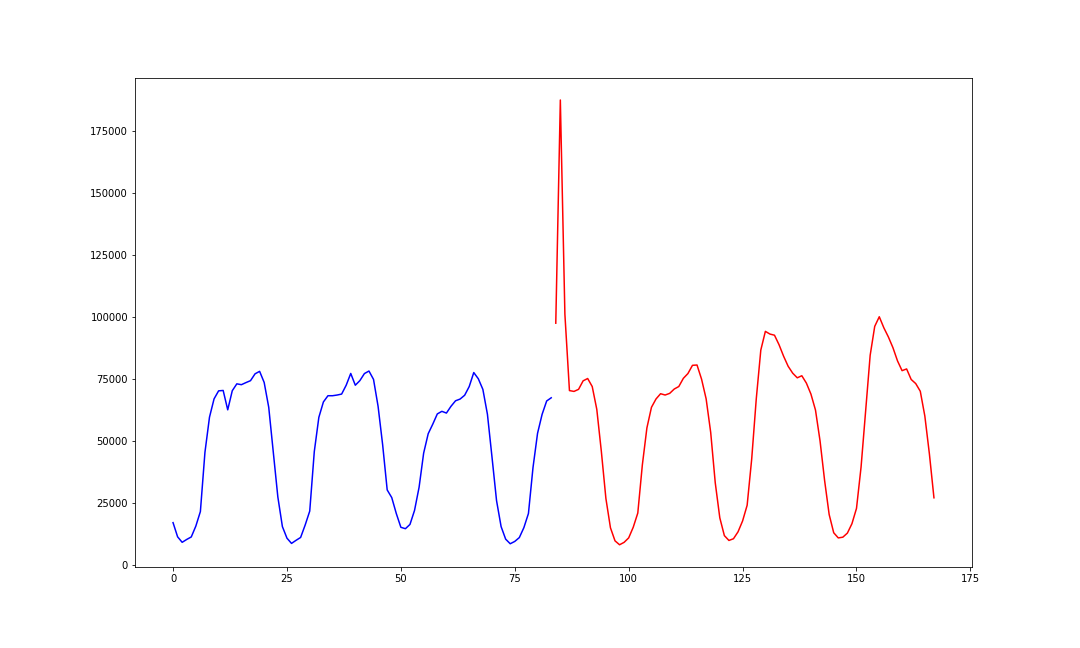
\includegraphics[scale=0.10]{images/022_point_cp_detected}
\end{figure}

Doesn't work for point change.
The reason is that we always move window from left to the right.

\end{frame}

\begin{frame}
    \frametitle{SSA in action. Point change}
    
Let's try to reverse the time series each time we find change point.

\begin{figure}
	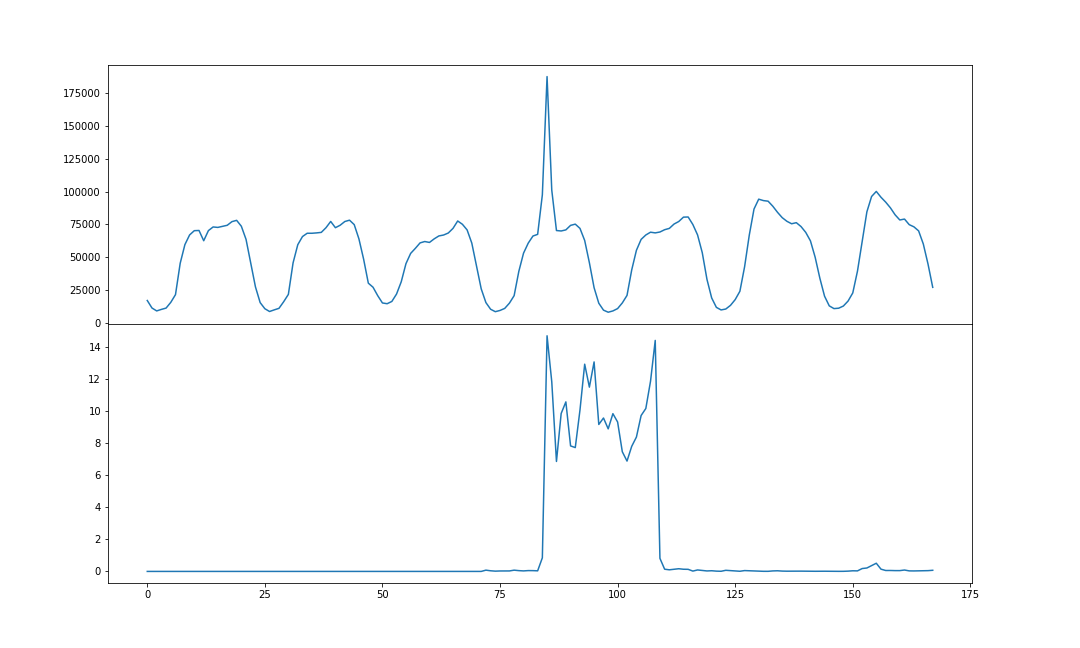
\includegraphics[scale=0.10]{images/023_point_cp_2}
	N = 48, L = 24, I = 5, p = 49, q = L, threshold = 0.1
	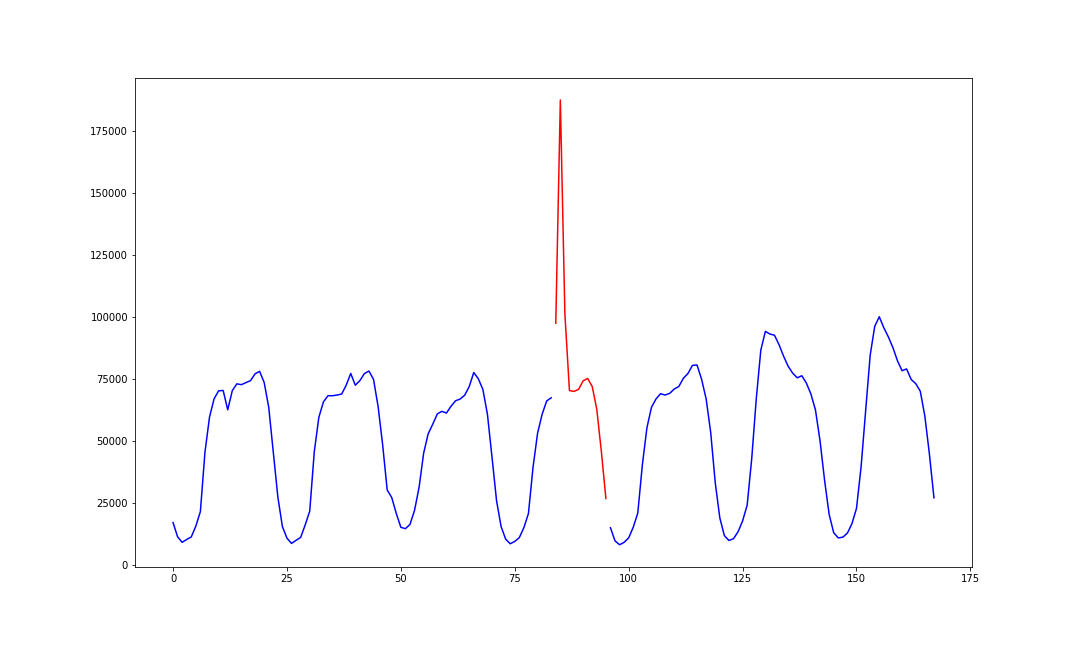
\includegraphics[scale=0.10]{images/024_point_cp_detected_2}
\end{figure}

Using this upgrade we make SSA algorithm working for point change as well

\end{frame}


\begin{frame}
    \frametitle{SSA in action. Parameters}
    
Now let's try to fit SSA parameters automatically for change point detection.

\end{frame}


\section{Airpush cases}

\begin{frame}
    \frametitle{Airpush cases. Fraud elimination}
    \begin{itemize}
    	\item Apps minutely requests data
	\item Red flag: strong pattern.
	\item Can be a automated bots behind pattern
    \end{itemize}
    \begin{figure}
	\textbf{Clean application}
	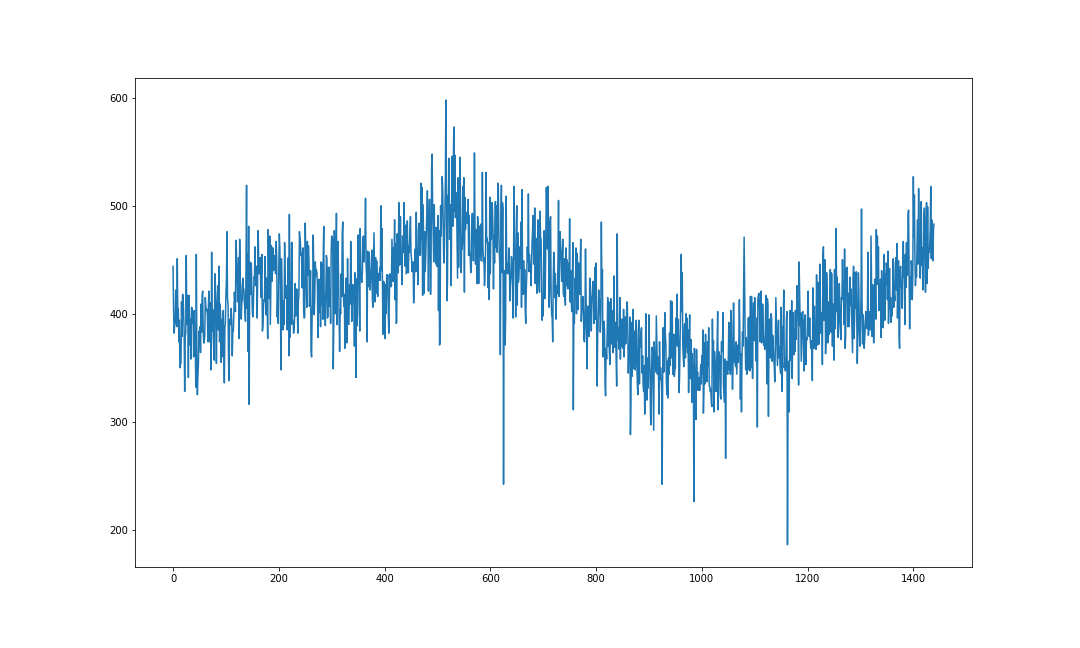
\includegraphics[scale=0.10]{images/007_case_1}
	\textbf{Fraud application}
	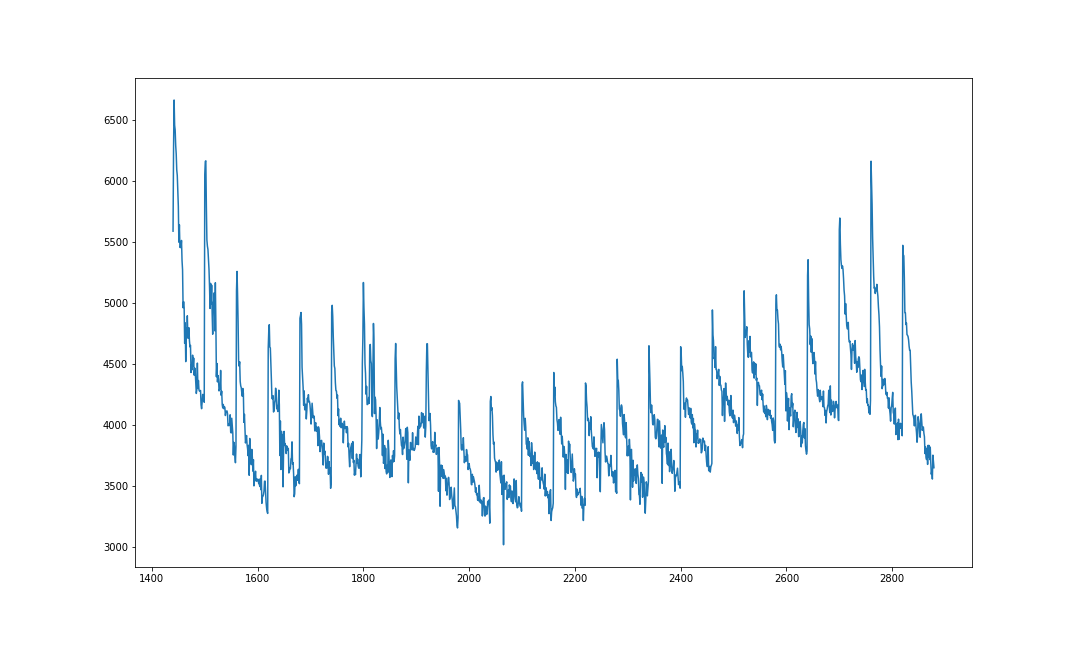
\includegraphics[scale=0.10]{images/008_case_1}
     \end{figure}
	
\end{frame}


\begin{frame}
    \frametitle{Airpush cases. Fraud elimination}
    \begin{itemize}
    	\item Goal: to be able to find such apps automatically
	\item We can reach this goal using frequency analysis
    \end{itemize}
    The framework can be described as follows:
   	 \begin{enumerate}
	 \item Apply logarithm to time series to stabilyze amplitude
 	 \item Remove trend (low frequent part) from time series
	 \item Apply Fourier transform to time series
	 \item Estimate the distribution of periodogram values
	 \item Compare distributions of each application with a distribution of white noise (which is exponential) using Kullback–Leibler divergence 
	 \item If divergence $>$ threshold, then application is marked as suspicious
	\end{enumerate}
\end{frame}



\begin{frame}
    \frametitle{Airpush cases. Fraud elimination}
    \framesubtitle{1. Apply logarithm}
    \begin{figure}
	\textbf{Clean application}
	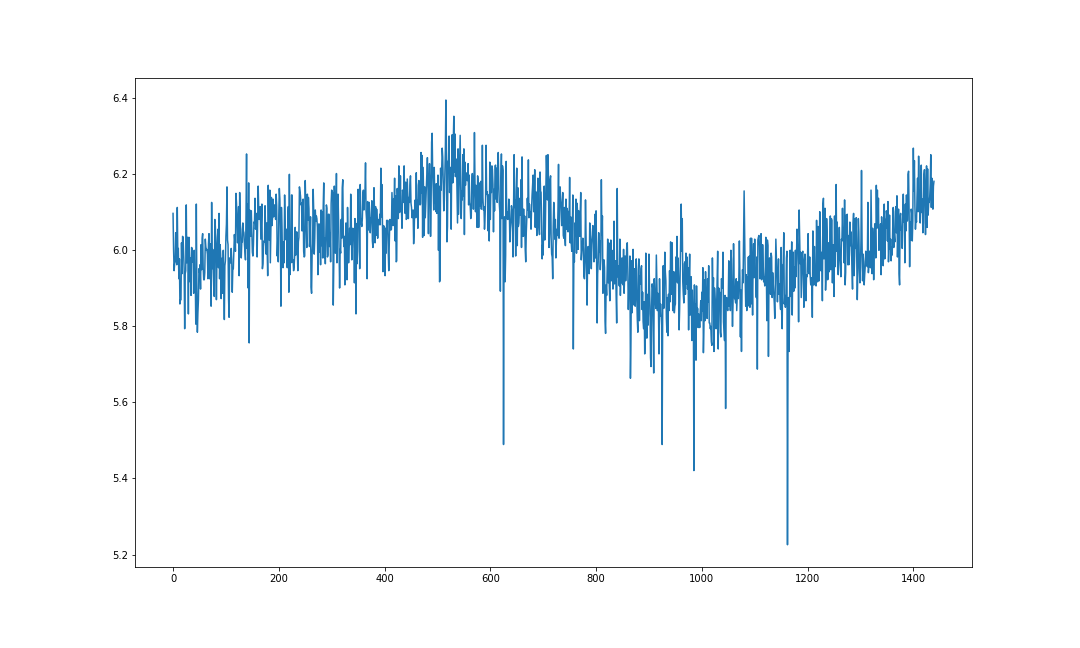
\includegraphics[scale=0.10]{images/009_case_1}
	\textbf{Fraud application}
	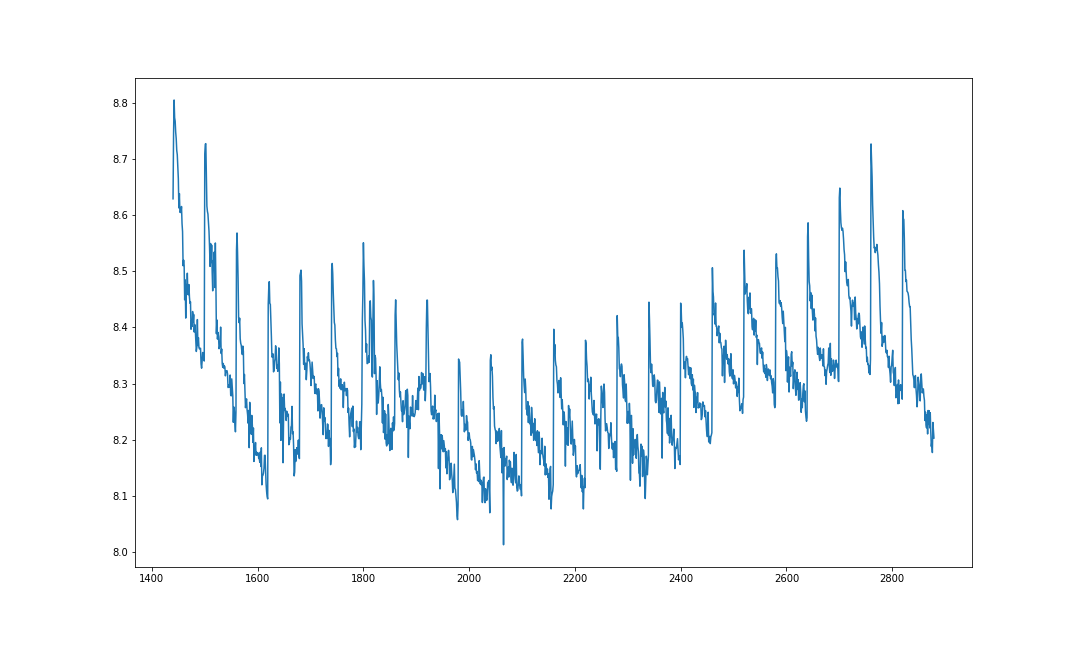
\includegraphics[scale=0.10]{images/010_case_1}
     \end{figure}
\end{frame}

\begin{frame}
    \frametitle{Airpush cases. Fraud elimination}
    \framesubtitle{2. Remove trend}
    \begin{figure}
	\textbf{Clean application}
	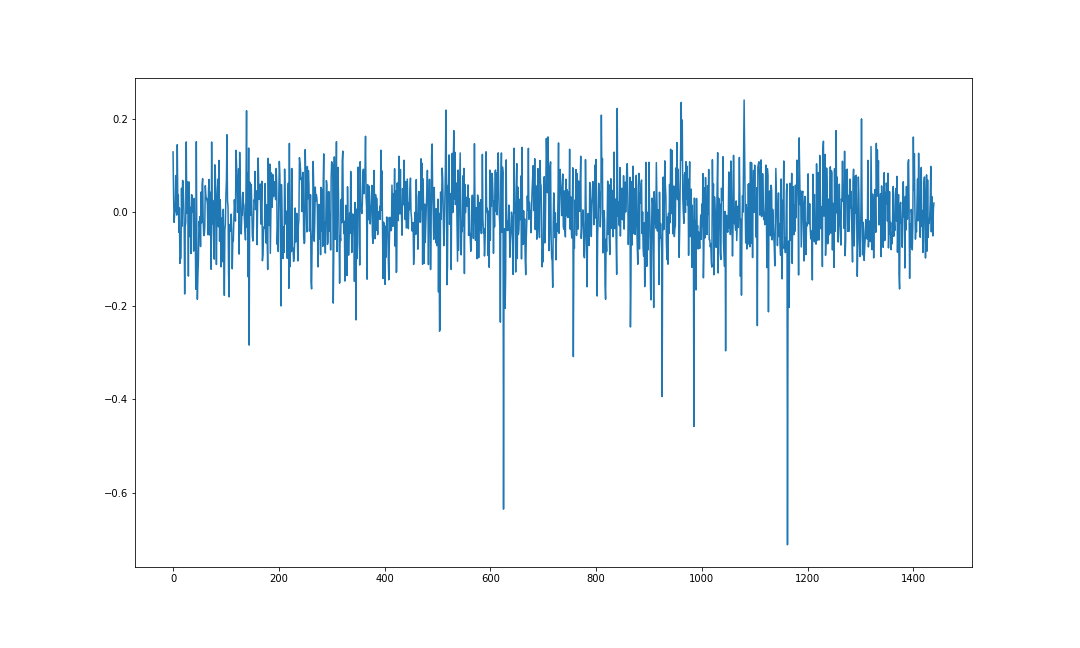
\includegraphics[scale=0.10]{images/011_case_1}
	\textbf{Fraud application}
	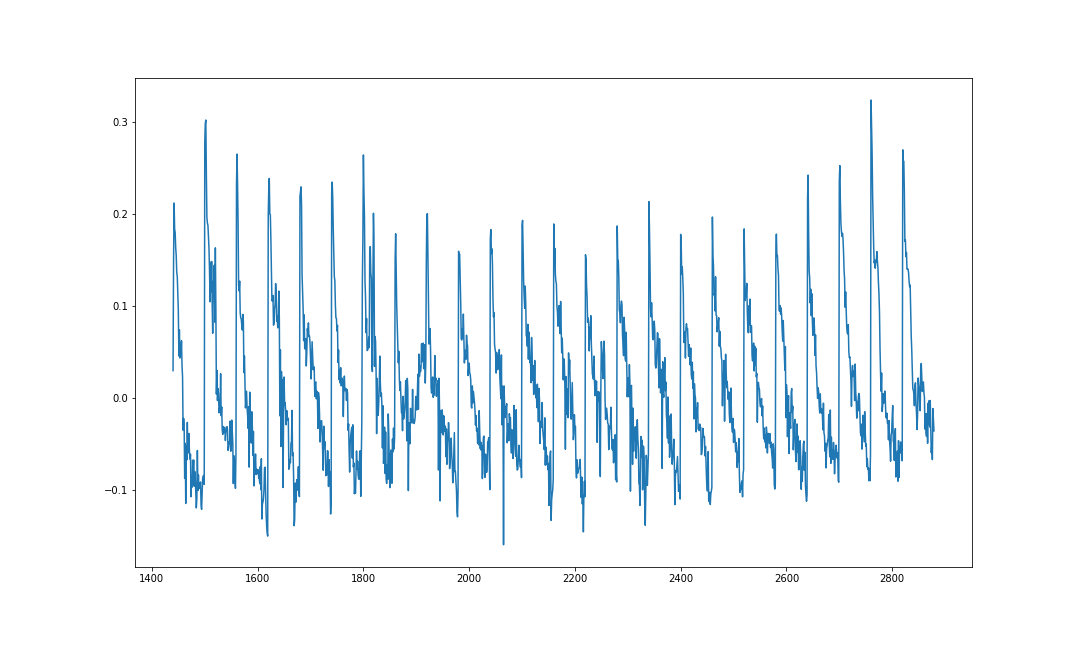
\includegraphics[scale=0.10]{images/012_case_1}
     \end{figure}
\end{frame}

\begin{frame}
    \frametitle{Airpush cases. Fraud elimination}
    \framesubtitle{3. Apply Fourier transform}
    \begin{figure}
	\textbf{Clean application}
	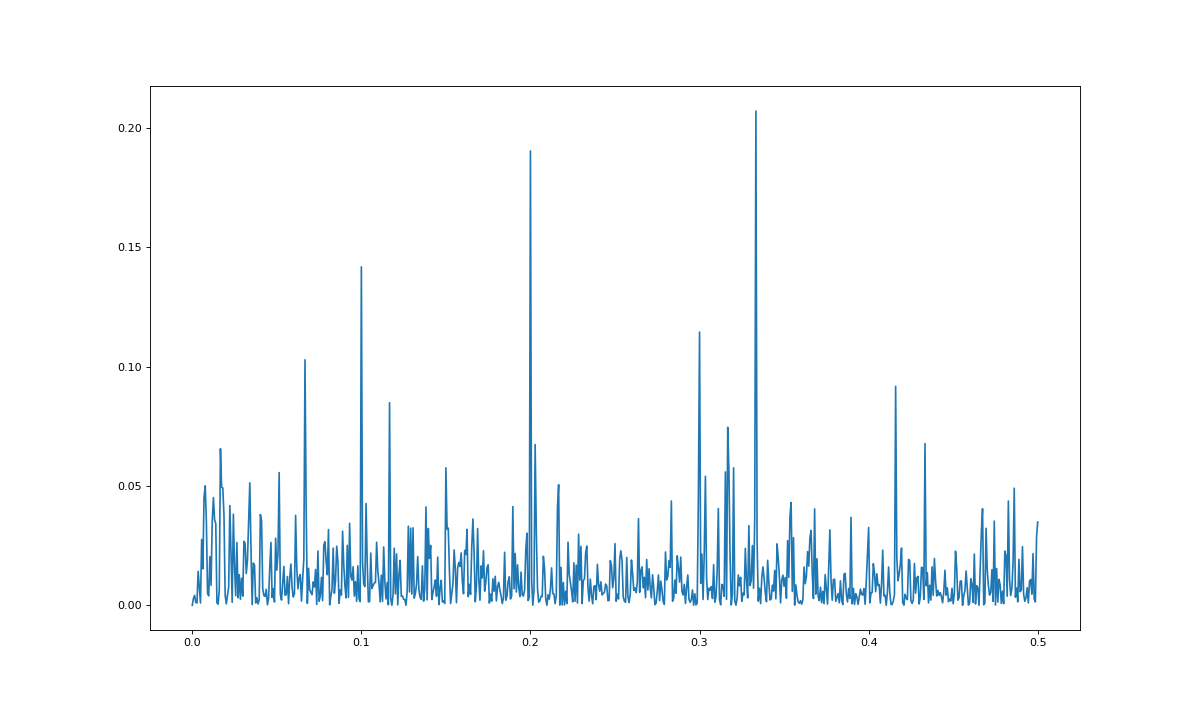
\includegraphics[scale=0.10]{images/013_case_1}
	\textbf{Fraud application}
	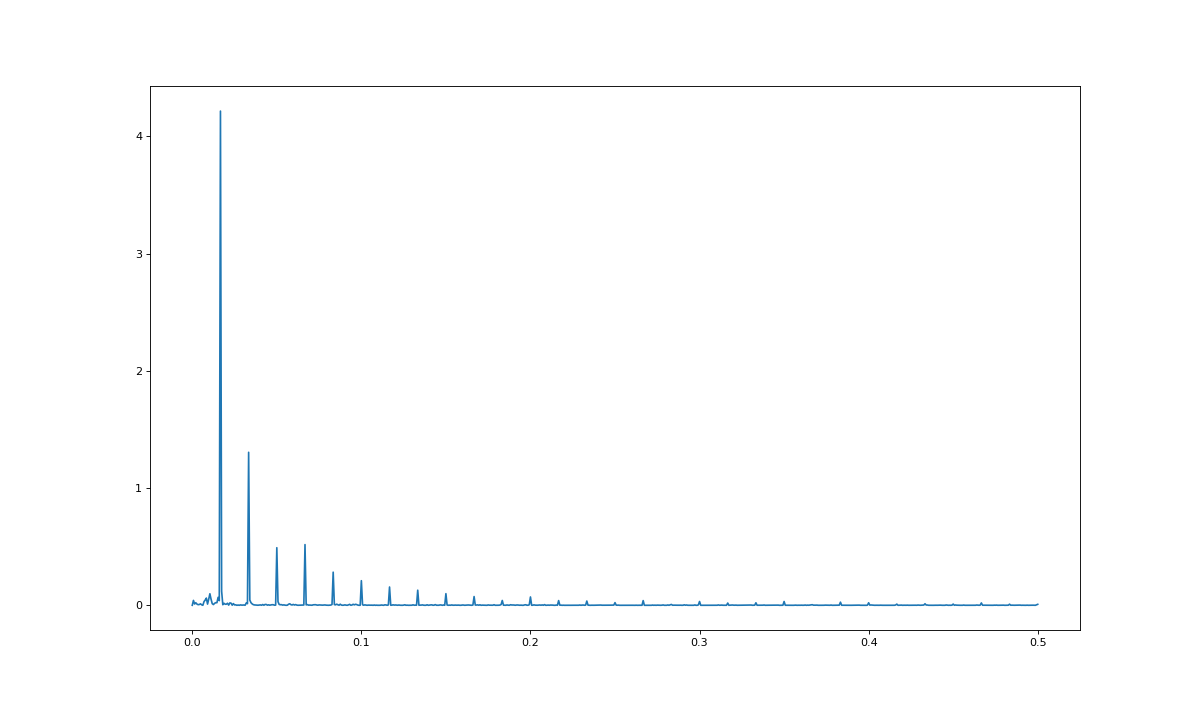
\includegraphics[scale=0.10]{images/014_case_1}
     \end{figure}
\end{frame}

\begin{frame}
    \frametitle{Airpush cases. Fraud elimination}
    \framesubtitle{4. Estimate the distribution of periodogram values}
    \begin{figure}
	\textbf{Clean application}
	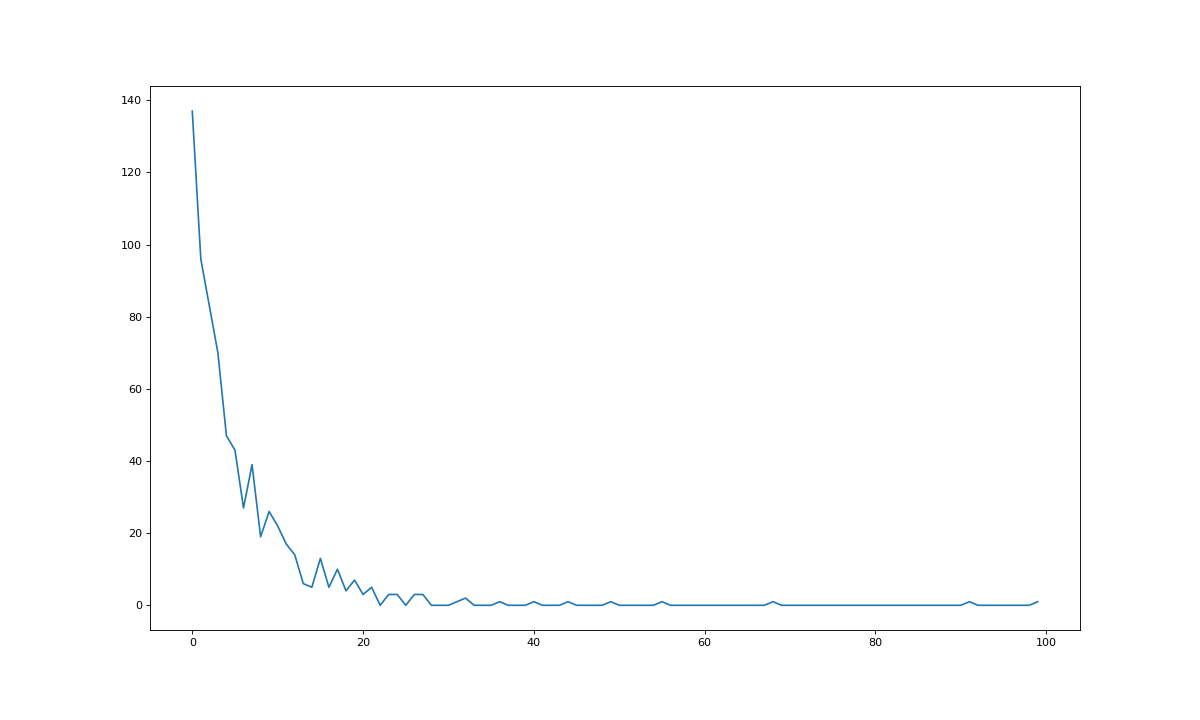
\includegraphics[scale=0.10]{images/015_case_1}
	\textbf{Fraud application}
	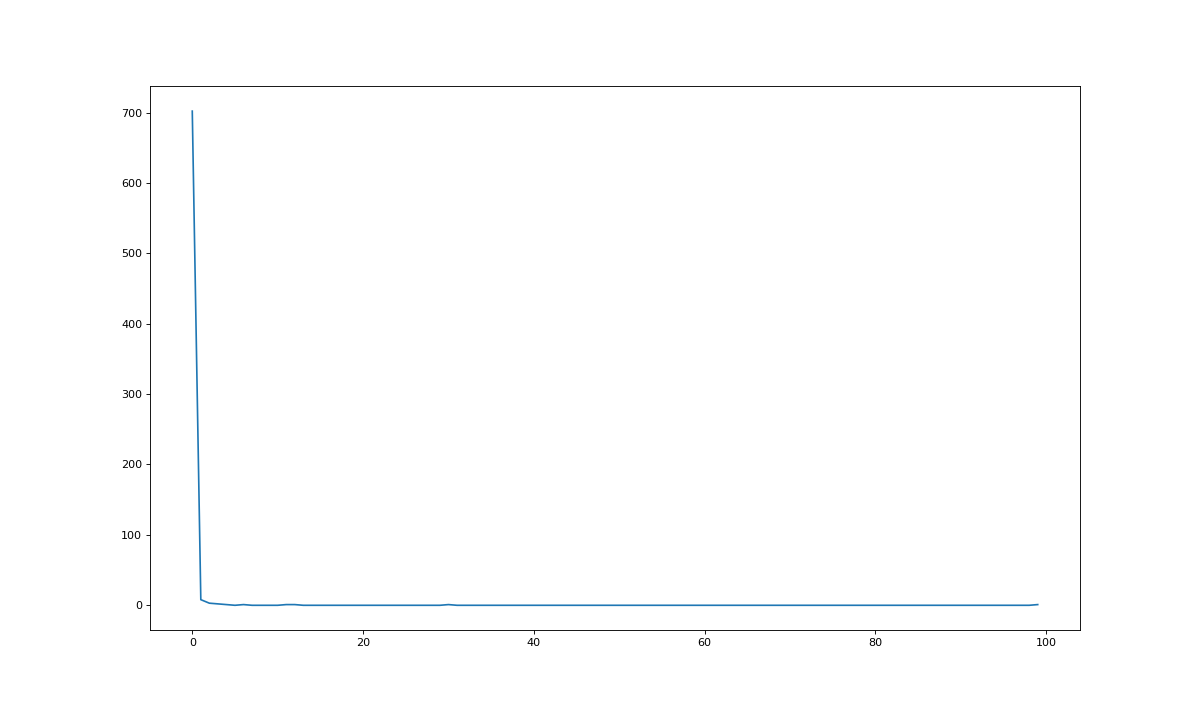
\includegraphics[scale=0.10]{images/016_case_1}
     \end{figure}
\end{frame}

\begin{frame}
    \frametitle{Airpush cases. Fraud elimination}
    \framesubtitle{5. Compare distributions}
    \begin{itemize}
    	\item Clean app score: 0.09
	\item Fraud app score: 1.87
    \end{itemize}
\end{frame}

\end{document}
